\section{Einleitung}
In dieser Versuchsreihe werden die Frequenzaufspaltungen von sichtbaren Licht aus verschiedenen Quellen untersucht. 

\subsection{Funktionsweise von Spektrometern}
Das Konzept aller Spektrometer ist Licht abhängig von der Wellenlänge verschieden abzulenken. Der Unterschied zwischen verschiedenen Spektrometern ist die Realisierung der Ablenkung. Abhängig davon ergeben sich verschiedene Wellenlängen-Winkel-Beziehungen. Im Versuch wurden zur Ablenkung Brechung am Prisma und Beugung am Gitter verwendet. Um die Auflösung zu verbessern wird das einfallende Licht kollimiert und durch einen Spalt fokussiert. Um die Ablenkung genauer zu messen wird ein Fernrohr verwendet.
\subsubsection{Prismenspektrometer}
In diesem Spektrometer wird die Brechung am Prisma genutzt. Da der Brechungsindex für Licht mit kürzerer Wellenlänge zunimmt wird blaues Licht stärker gebrochen als rotes Licht. Es entsteht somit eine Frequenzaufspaltung, bei der außen Licht mit geringster Wellenlänge und höchster Frequenz zu sehen ist, während innen Licht mit zunehmend größerer Wellenlänge und geringerer Frequenz zu sehen ist.
\subsubsection{Gitterspektrometer}
Bei der Beugung am Gitter treten die Beugungsmaxima Wellenlängenabhängig auf. Es lässt sich zwischen Winkel des Maxima $ \vartheta $, Wellenlänge des Lichts $ \lambda $, Gitterkonstante des verwendeten Gitters $ g $ und Ordnung des Maxima $ m $ der folgende Zusammenhang herleiten:
\begin{equation}
	\lambda = \frac{g\sin\vartheta_m}{m} \label{eq:theo:beug}
\end{equation}
Mit einem Gitterspektrometer sind nicht beliebig kleine Wellenlängenauflösungen möglich. Das  Rayleigh-Kriterium besagt, dass eine Unterscheidung gerade noch möglich ist, falls das Maximum der einen mit dem Minimum der anderen Wellenlänge zusammenfällt. Daraus folgt für den minimalen Wellenlängenunterschied $ \Delta \lambda $ bei mittlerer Wellenlänge $ \lambda $, Anzahl der beleuchteten Gitterspalte $ N $ und Ordnung $ m $ der Zusammenhang
\begin{equation}
	\Delta\lambda \geq \frac{\lambda}{mN}
\end{equation}
\subsection{Lichtspektren}
Abhängig von der Lichtquelle entstehen verschiedene Lichtspektren. Im allgemeinen wird unterschieden zwischen diskreten und kontinuierlichen Spektren. In kontinuierlichen Spektren treten alle Wellenlängen eines Wellenlängenbereiches auf. Bei diskreten Spektren treten dagegen nur einzelne Frequenzen auf. Im Spektrometer äußert sich dies in einem Linienspektrum. Es sind  scharf abgegrenzte, helle Linien zu erkennen, während der Bereich dazwischen dunkel bleibt. Innerhalb eines kontinuierlichen Spektrums sind dagegen kontinuierliche Farbverläufe zu erkennen. 
\subsubsection{Gasentladung}
Bei Lichterzeugung durch Gasentladung entstehen diskrete Spektren. Die Elektronen in der Schale der Gasatome können nur auf diskreten Bahnen angeregt werden. Daher kann nur Licht mit diskreten Energiewerten $ \Delta E $ ausgesendet werden. Da sich die Wellenlängen $ \lambda $ direkt aus der Energie ergeben sind auch diese diskret verteilt. Es gilt
\begin{equation}
	\Delta E = \frac{hc}{\lambda}
\end{equation}
$ hc $ ist das Produkt aus Plankschen Wirkungsquantor $ h $ und Vakuumlichtgeschwindigkeit $ c $.

\subsubsection{Glut}
Erhitzte Körper geben ein kontinuierliches Strahlenspektrum ab. Ab Temperaturen von etwa \SI{600}{\degreeCelsius} verschiebt sich das Spektrum in den Bereich des sichtbaren Lichtes. Mit zunehmender Temperatur wird der Anteil von kurzwelligen Licht geringer. Lichtquellen, bei denen das Licht durch diesen Effekt erzeugt wird sind unter Anderem Glühbirnen und die Sonne. Jedoch entspricht das Spektrum der Sonne nicht vollständig dem kontinuierlichen Modell. Analog zur Emission bei Gasentladung kommt es durch Atome im äußeren Bereich der Sonne zu Absorption derselben Frequenzen. Somit sind im Sonnenspektrum schwarze Linien erkennbar. Diese werden als Fraunhoferlinien bezeichnet.

\subsection{Leuchtdioden}
Beim \textit{pn}-Übergang in Dioden müssen Elektronen das elektrische Potential der Raumladungszone überwinden. Dabei erhält die Diode die Energie $ E_G = U \cdot e $. Diese wird in Form eines Lichtquants abgegeben. Analog zur Gasentladung gilt
\begin{equation}
	E_G = U\cdot e = \frac{hc}{\lambda} \label{eq:theo:diode}
\end{equation}
Da die Energie der freien Elektronen keine diskreten Werte annimmt kommt es zu einem kontinuierlichen Strahlenspektrum in einem kleinen Wellenlängenbereich. Von Leuchtdioden ausgesandtes Licht ist nahezu monochromatisch. Die Wellenlänge $ \lambda $ der maximalen Intensität ist antiproportional zur Energie $ E_g $ und somit auch zur Spannung $ U $
\newpage
\section{Auswertung}
\subsection{Prisma und Gitter}
Wird das Prisma als optische Komponente im Spektrometer verwendet und so ausgerichtet, dass der Strahlengang symmetrisch ist. Der Spalt wird mit einer  Natriumdampflampe ausgeleuchtet. Es sind wie erwartet zwei Linien sichtbar. Diese Linien waren aber nicht gerade sondern leicht gekrümmt, was auf eine nicht ganz richtige Ausrichtung des Spektrometers zurückzuführen ist.
Wird das Prisma durch das Transmissionsgitter mit $ g=\SI{1/300}{\milli\meter} $  ersetzt, sind Linien bis zur 4 Beugungsordnung auffindbar. Dabei ist auffällig, dass je höher die Beugungsordnung wird, desto mehr war erkennbar, dass es sich um zwei sich überschneidende Linien handelt. Diese sind nicht scharf unterscheidbar.
\begin{tabular}{|c|c|c|}
\hline 
Beugungsordnung & Lage der Hauptmaxima links & Lage der Hauptmaxima rechts \\ 
\hline 
0 & 0 & 0 \\ 
\hline 
1 & 10 & 349,75 \\ 
\hline 
2 & 20,5 & 339,5 \\ 
\hline 
3 & 31,75 & 328,25 \\ 
\hline 
4 & 44,5 & 315,25 \\ 
\hline 
\end{tabular} 
Die Fehler für die Gradzahlen betragen $ \pm 0,25 $.
Wird das Transmissuinsgitter mit einem ausgetauscht, dessen Gitterkonstante $ g=\SI{1/600}{\milli\meter} $ so ist zu beobachten, dass die Hauptmaxima weiter auseinander gehen ( Abstände verdoppeln sich) und das die Intensität stärker abnimmt.

\subsection{Quantitative Untersuchung verschiedener Spektren am Gitterspektrometer}
Im zweiten Versuchsteil werden die Lichtspektren verschiedener Lichtquellen an einem Gitterspektrometer untersucht. Im Spektrometer wird ein Gitter mit der Gitterkonstante $ g = \SI[quotient-mode=fraction]{1/600}{\milli\meter} $ verwendet. Die verwendeten Lichtquellen sind
\begin{itemize}
\item Energiesparlampe
\item Leuchtdioden in den Farben
\begin{itemize}
	\item rot
	\item gelb
	\item grün
	\item blau
\end{itemize}
\end{itemize}
\subsubsection{Kalibrierung des Spektrometers}
Um das Spektrometer zu kalibrieren wird zunächst das Licht einer Heliumdampflampe untersucht. Da aus der Versuchsanleitung \cite{anleitung2015} die Wellenlängenaufspaltung bekannt ist, lässt sich damit ein Zusammenhang zwischen Beugungswinkel und Wellenlänge aufstellen. Die von uns gesehenen Spektrallinien sind in Tabelle \ref{tab:kalib} zu finden.\\
\begin{table}[H]
\centering\
\sisetup
{
	table-figures-integer = 1,
	table-figures-decimal = 3,
	table-figures-uncertainty = 3,
	table-number-alignment= center
}
\begin{tabular}{cS[table-format=3.1]SS}
Farbe & {Wellenlänge [\si{\nano\meter}]} & {Beugungswinkel $ \vartheta $ [\si{\radian}]} & {$ \sin\vartheta $} \\\hline\hline
indigo & 438.8 & 0,262 +- 0,005 & 0.259 +- 0.005 \\
indigo & 447.1 & 0,271 +- 0,005 & 0.267 +- 0.005 \\
blau & 471.3 & 0,281 +- 0,005 & 0.277 +- 0.005 \\
grünblau & 492.2 & 0,298 +- 0,005 & 0.294 +- 0.005 \\
grün & 501.5 & 0,310 +- 0,005 & 0.305 +- 0.005 \\
gelb & 587.5 & 0,358 +- 0,005 & 0.350 +- 0.005 \\
rot & 667.8 & 0,410 +- 0,005 & 0.399 +- 0.005 \\
rot & 706.5 & 0,441 +- 0,005 & 0.427 +- 0.004
\end{tabular}
\caption{Spektrallinien der Heliumdampflampe im Spektrometer}
\label{tab:kalib}
\end{table}

Aus dem in der Theorie gegebenen Zusammenhang \eqref{eq:theo:beug} wird $ \sin\vartheta \propto \lambda $ erwartet. Daher wird die Formel
\begin{equation}
	\lambda = a\cdot \sin\vartheta \label{eq:kalib}
\end{equation}
aufgestellt. Der Proportionalitätsfaktor $ a $ wird dabei mithilfe von \textit{Gnuplot\footnote{Version 4.6 patchlevel 4 unter Linux x86\_64 \url{http://sourceforge.net/projects/gnuplot/files/gnuplot/4.6.4/}}} nach dem \textit{Least-Squares-Fit} verfahren bestimmt. Grafisch dargestellt ist dies in Abbildung \ref{fig:kalib}. Der so bestimmte Proportionalitätsfaktor beträgt $ a = \SI{1672+-6}{\nano\meter}$ 

\begin{figure}[H]
	\centering
	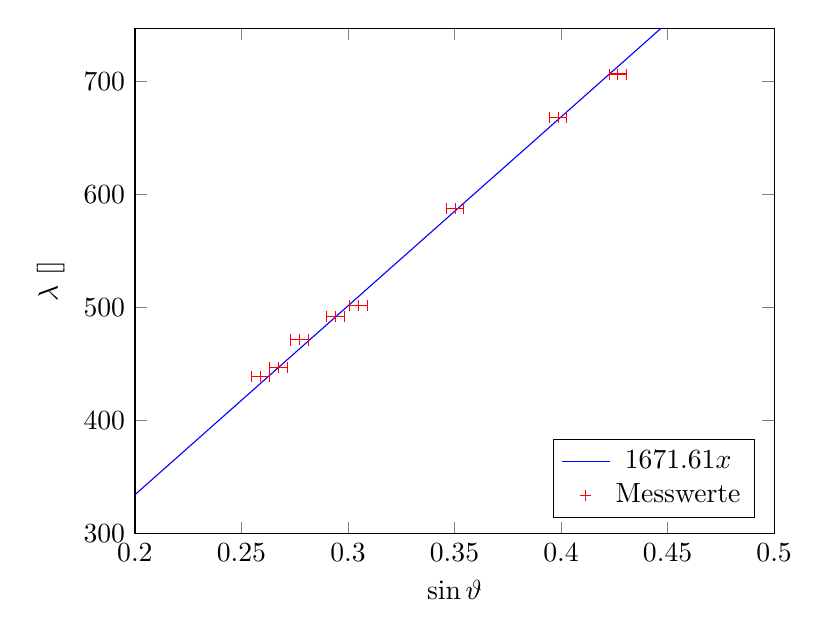
\begin{tikzpicture}
\begin{axis}[xmin = 0.2, ymin = 300, xmax = .5,
	legend pos = south east, width = .8\textwidth, height = 8cm,
	xlabel = $ \sin\vartheta $,
	ylabel = {$ \lambda $ [\si{\nano\meter}]}]
	
	\addplot+[no marks, ] {1671.61*x};
	\addplot+[mark = +,only marks, error bars/.cd, x dir = both, x explicit,] table[x=x,y=y, x error = xerr] {
y	x	xerr
438.8	0.2588190451	0.0042146465
447.1	0.2672383761	0.004204631
471.3	0.2773146533	0.0041921899
492.2	0.2940403252	0.0041704338
501.5	0.304864299	0.0041556106
587.5	0.3502073813	0.0040870034
667.8	0.3987490689	0.0040014294
706.5	0.4265687399	0.0039464301
};
\legend{{$ \num{1671.61}x $}, Messwerte}
\end{axis}
\end{tikzpicture}
	\caption{Eichkurve}
	\label{fig:kalib}
\end{figure}

\subsubsection{Spektrum der Energiesparlampe}
In diesem Versuchsteil wird das Spektrum einer Energiesparlampe mit dem zuvor kalibrierten Spektrometer untersucht. Damit und mit der bei der Kalibration bestimmten Formel \eqref{eq:kalib} lässt sich das Wellenlängenspektrum bestimmen. Die von uns bestimmten Werte sind Tabelle \ref{tab:espar} zu entnehmen. Zur Berechnung der Fehler wurden \eqref{eq:err:sin} und \eqref{eq:err} verwendet.

\begin{table}[H]
	\centering
	\sisetup{table-figures-integer = 1,
		table-figures-decimal = 3,
		table-figures-uncertainty=3,
		table-number-alignment = center}
	\begin{tabular}{cSSS[table-format=3+-1]}
	Farbe & {Beugungswinkel $ \vartheta $ [\si{\radian}]} & {$ \sin\vartheta $} & {Wellenlänge $ \lambda $ [\si{\nano\meter}]}\\\hline\hline
	rot & 0,428 +- 0,004 & 0,415 +- 0,004 & 693 +- 6 \\
	rot & 0,417 +- 0,004 & 0,405 +- 0,004 & 677 +- 6 \\
	rot & 0,398 +- 0,004 & 0,388 +- 0,004 & 648 +- 6 \\
	rot & 0,382 +- 0,004 & 0,373 +- 0,004 & 623 +- 6 \\
	orange & 0,370 +- 0,004 & 0,362 +- 0,004 & 604 +- 6 \\
	orangegelb & 0,360 +- 0,004 & 0,352 +- 0,004 & 588 +- 6 \\
	orangegelb & 0,358 +- 0,004 & 0,350 +- 0,004 & 585 +- 6 \\
	orangegelb & 0,356 +- 0,004 & 0,349 +- 0,004 & 583 +- 6 \\
	gelb & 0,349 +- 0,004 & 0,342 +- 0,004 & 572 +- 6 \\
	grün & 0,332 +- 0,004 & 0,326 +- 0,004 & 544 +- 6 \\
	blau & 0,297 +- 0,004 & 0,292 +- 0,004 & 489 +- 6 \\
	indigo & 0,271 +- 0,004 & 0,267 +- 0,004 & 447 +- 6 \\
	violett & 0,246 +- 0,004 & 0,244 +- 0,004 & 407 +- 6
	\end{tabular}
	\caption{Spektrallinien der Energiesparlampe}
	\label{tab:espar}
\end{table}

\subsubsection{Spektrum der Dioden}
Im letzten Versuchsteil wird das Spektrum von Dioden untersucht. Dazu wird weiterhin das kalibrierte Spektrometer verwendet, so dass \eqref{eq:kalib} weiter als Beugungswinkel-Wellenlängen-Beziehung verwendet werden kann. Bei Dioden ist insbesondere die Einschaltspannung von besonderer Bedeutung, da diese der Potenzialbarriere der Raumladungszone entspricht. Diese kann dann mit der Wellenlänge der maximalen Intensität in einen Zusammenhang gebracht werden.\\
Anders als bei der Energiesparlampe konnten wir hier kein diskretes Spektrum beobachten. Stattdessen waren kontinuierliche Spektren über verhältnismäßig kleine Wellenlängenbereiche zu erkennen. Da es mit dem Auge schwer möglich ist Intensitäten verschiedener Lichtfarben zu vergleichen sind Winkel, unter denen die Maxima auftreten nicht genau messbar. Wir erhielten für die vier Leuchtdioden mit den Lichtfarben rot, gelb, grün und blau die Wellenlängenmaxima und Einschaltspannungen aus Tabelle \ref{tab:diode}. Die Fehler wurden mit \eqref{eq:err} und \eqref{eq:err:sin} bestimmt.

\begin{table}[H]
\centering
\begin{tabular}{cSSS}
	Farbe & {Einschaltspannung $ U $ [\si{\volt}]} & {Maximumswinkel $ \vartheta $ [\si{\radian}]} & {Wellenlänge $ \lambda $ [\si{\nano\meter}]} \\\hline\hline
	rot & 1,36 +- 0,01 & 0,367 +- 0,005 & 613 +- 8 \\
	gelb & 1,48 +- 0,01 & 0,345 +- 0,005 & 576 +- 8 \\
	grün & 1,57 +- 0,01 & 0,332 +- 0,005 & 554 +- 8 \\
	blau & 2,35 +- 0,01 & 0,236 +- 0,005 & 394 +- 8
\end{tabular}
\caption{Einschaltspannungen und Wellenlängenmaxima der Leuchtdioden}
\label{tab:diode}
\end{table}
Nach \eqref{eq:theo:diode} ist $ U\cdot e \propto \frac{1}{\lambda} $ zu erwarten mit Proportionalitätskonstante $ a = hc $. Der Proportionalitätsfaktor $ a $ wird mithilfe von \textit{Gnuplot\footnote{Version 4.6 patchlevel 4 unter Linux x86\_64 \url{http://sourceforge.net/projects/gnuplot/files/gnuplot/4.6.4/}}} nach dem \textit{Least-Squares-Fit} verfahren bestimmt.

\begin{figure}[H]
\centering
\begin{tikzpicture}
\begin{axis}[ xmin = 1.5, ymin = 1.3, xmax = 2.6, ymax = 3,
	legend pos = south east, width = .8\textwidth, height = 8cm,
	xlabel = {$ \frac{1}{\lambda}~[\si{\per\micro\meter}] $},
	ylabel = {$ U\cdot e $ [\si{\electronvolt}]}]
	
	\addplot+[no marks, ] {0.917936*x};
	\addplot+[no marks, ] {1.243*x};
	\addplot+[mark = +,only marks, error bars/.cd, x dir = both, x explicit,y dir = both, y explicit] table[x=x,y=y, x error = xerr, y error = yerr] {
y	yerr	x	xerr
1.36	0.01	1.6321812223	0.0202823427
1.48	0.01	1.7354838313	0.0228218387
1.57	0.01	1.803989772	0.0245915894
2.35	0.01	2.2850537112	0.0389447822
};
\legend{{$ \num{0,918}\frac{1}{\lambda} $ (Fit)}, {$ \num{1,240}\frac{1}{\lambda} $ (Theorie)} , Messwerte}
\end{axis}
\end{tikzpicture}
\caption{}
\label{fig:diode}
\end{figure}
Gnuplot liefert uns den Proportionalitätsfaktor $ a = hc = \SI{.92(5)}{\electronvolt\micro\meter} = \SI{920(50)}{\electronvolt\nano\meter} $


\newpage
\section{Diskussion} 
\subsection{Verschiedene Beugungsgitter}
Beim Vergleich der beiden Beugungsgitter mit $ g = \SI{1/300}{\milli \meter} $ und $ g = \SI{1/600}{\milli\meter} $ fällt zunächst auf, dass bei dem zweiten Gitter weniger Maxima zu erkennen sind. Bei genauerer Betrachtung ist zu erkennen, dass die Maxima des zweiten Gitters jeweils einem Maximum doppelter Ordnung des ersten Gitters entsprechen. Diesen Zusammenhang hätte man sich in der Theorie auch aus \eqref{eq:theo:beug} einfach herleiten können: Verdoppelt man sowohl die Beugungsordnung als auch die Gitterkonstante kürzen sich die beiden Verdoppelungen aus der Gleichung und es bleibt der gleiche Wellenlängen-Beugungswinkel-Zusammenhang bestehen.
\subsection{Auflösungsvermögen}
Vergleicht man die Spektren der verschiedenen dispergierenden Elemente, so ist der auffälligste Unterschied, dass beim Prisma zwei scharf trennbare Linien sichtbar sind. Bei den Gittern sind mit zunehmender Beugungsordnung zwei sich überschneidende Linien zu erkennen, daraus ist zu schließen, dass der Wellenlängenunterschied zu gering ist, um scharfe Linien aufzulösen.
Dieser beträgt bei der verwendeten Natriumdampflampe $ \SI{0,6}{\nano\meter} $. Die Gitter unterscheiden sich durch ihre Spaltenanzahl, daraus ergibt sich wie nach dem Rayleigh-Kriterium eine bessere Unterscheitbarkeit der sich überschneidenden Linien. 


\subsection{Spektrum der Energiesparlampe}
Im Gegensatz zur Natriumdampflampe zeigt die Energiesparlampe einen deutlich umfangreicheres Spektrum. Dieses hat zum einen mehr Spektrallinien und ist zum anderen über einen breiteren Wellenlängenbereich verteilt. Dies ist wichtig um ein möglichst weißes Licht zu erzeugen. Weißes Licht kann nicht monochromatisch sein sondern wird immer aus Mischung mehrerer Lichtfarben erzeugt.\\
Zudem fällt auf, dass die Mehrheit der Spektrallinien im Bereich des roten, längerwelligen Lichtes liegt. Dies ist eine erwünschte Eigenschaft, da rotes Licht im allgemeinen als warm empfunden wird, während blaues Licht als kalt wahrgenommen wird. \\
Wir nehmen an, dass als Füllgas Quecksilberdampf verwendet wird. Vergleicht man das von uns erfasste Spektrum mit dem Hg II Spektrum \cite{NIST_ASD} findet man sehr intensive Spektrallinien bei Wellenlängen $ \lambda $ von \SIlist{588,9; 587.1;567.7;542.5}{\nano\meter}. Wir haben durch unsere Messungen unter anderem Spektrallinien bei \SIlist{588(6);585(6);572(6);544(6)}{\nano\meter}

\subsection{Spektren der Dioden}
Der erwartete Zusammenhang zwischen Spannung und Wellenlänge ließ sich nicht vollständig nachweisen. Zwar ist der antiproportionale Zusammenhang zwischen Wellenlänge und Spannung insbesondere für die rote, gelbe und grüne Diode gut zu erkennen, jedoch weicht die blaue Diode davon deutlich ab. Zudem liegt die Proportionalitätskonstante aus der Theorie gut \SI{40}{\percent} über der von uns bestimmten. \\
Dass diese Fehler auftreten lässt insbesondere mit der Art der Durchführung begründen. Mit dem Auge ist es allgemein nur subjektiv möglich Lichtintensitäten wahrzunehmen und zu vergleichen. Insbesondere Licht verschiedener Farben in ihrer Intensität zu vergleichen fällt sehr schwer. Beispielweise wird gelb als hellere Farbe wahrgenommen als rot. Da diese beiden Farben im Spektrum direkt nebeneinander Liegen kann es so schnell zu Fehlwahrnehmungen kommen. \\
Eine andere Eigenschaft der Dioden ließ sich dagegen gut bestätigen. Das ausgesendete Licht stammt aus einen kleinen Wellenlängenbereich. Dies ist auch in der Theorie nicht anders erwartet.